\problemname{Köpa matta}
\begin{center}
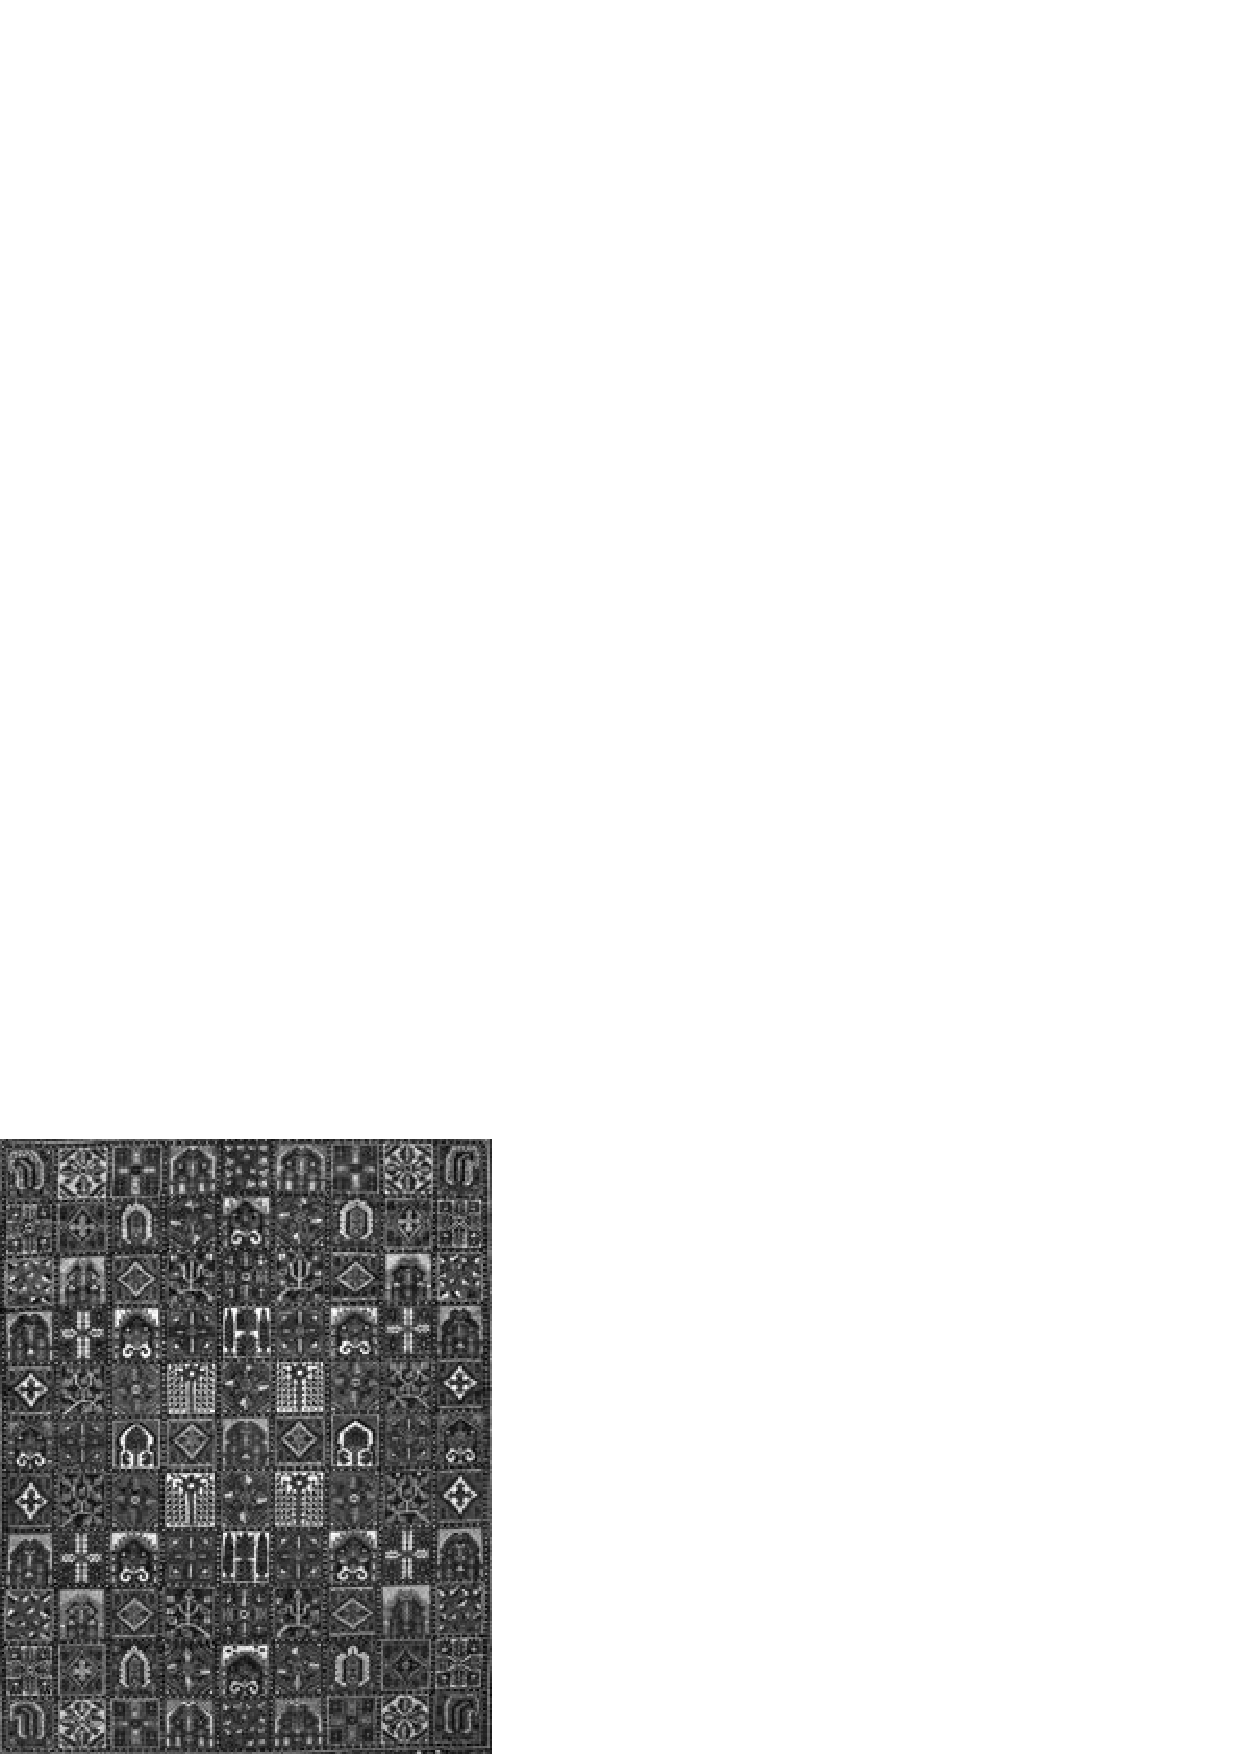
\includegraphics[width=4cm]{matta.pdf}
\end{center}

Under IOI i Teheran i somras märktes en ökad efterfrågan på persiska
mattor, i synnerhet sådana vars mönster utgörs av ett rutmönster med $L
\times B$ rutor (se bild ovan), eftersom dessa är mycket lämpliga för att i
hemlighet prova ut algoritmer på.

En mattas pris brukar avgöras av antalet rutor, så en typisk kund vill
ha en matta med minst $M$ rutor och högst $N$ rutor. Om det finns flera
möjliga mattor vill kunden ha en så kvadratisk matta som möjligt,
d.v.s. den vill att $|L - B|$ är så litet som möjligt.

Skriv ett program som läser in talen $M$ och $N$ och skriver ut det
bästa valet av $B$ och $L$.

\section*{Indata}

En rad med två heltal $M$ och $N$.

\section*{Utdata}

Skriv ut talen $B$ och $L$ (den minsta sidlängden först). För givna indata är svaret unikt bestämt.

\section*{Poängsättning}
För testfall värda $40$ poäng gäller att $1 \le M \le N \le 1\,000$ \\
För testfall värda $20$ poäng gäller att $M = N$, och $10^{11} \le M \le 10^{12}$ \\
För testfall värda $40$ poäng gäller att $10^8 \le M \le N \le 10^{12}$ \\
